\documentclass[12pt,a4paper]{article}
\usepackage{setspace}
\usepackage{hyperref,enumerate,float,amsfonts,amssymb,amsmath,graphics,graphicx}
\usepackage[margin=1.5 cm]{geometry}
%\usepackage[paperheight=22.5cm,paperwidth=15.75cm,margin=1.5 cm]{geometry}
\usepackage[none]{hyphenat}
\usepackage{wrapfig}
\usepackage{subfig}
\usepackage{fancyhdr}
\usepackage{color,soul}
\usepackage{lipsum}
\usepackage{tabularx}
\usepackage{romannum}
\AtBeginDocument{\pagenumbering{arabic}}
\newcounter{question}
\setcounter{question}{0}


\newcommand{\set}[1]{\setlength\itemsep{#1em}}
%\parindent 0ex
\parskip 0.3em



\newcommand\Que[1]{
   \line(1,0){300}
   \leavevmode\par
   \stepcounter{question}
   \noindent
   \fbox{\thequestion. Q} --- \hl{#1}\par}

\newcommand\Ans[2][]{%
    \leavevmode\par\noindent
   {\leftskip16pt
    A --- \textbf{#1}#2\par}}














\onehalfspacing

\begin{document}

\begin{titlepage}
\begin{center}
\vspace*{0.5cm}
EEC 232 Solid State: Physics and Devices
\vfill
\line(1,0){500}\\
\Huge{Chapter 2} \\
\line(1,0){500}\\
\vfill
{\LARGE Eng. Mina Mounir\footnote{{\normalsize \LaTeX\ by Taha Ahmed}}}
\vfill


\end{center}

\end{titlepage}

\begin{large}




\Que{Compare between electrons in isolated atoms and electrons in solids}
\Ans{
\begin{itemize}


\item Electrons in isolated atoms are restricted to sets of discrete energy levels\\
\item Electrons in solids are restricted to bands of available energies and are not allowed at others 
\end{itemize}
}

\Que{Illustrate the bonding forces in solids}
\Ans{

\begin{enumerate}
\item \textbf{The ionic bonding} : bonds between positive and negative ions.

\item \textbf{The metallic bonding} : The outer electron in each atom is contributed to the crystal as a whole so that the solid is made up ions with closed shells immersed in a sea of electrons. \\ The forces holding the lattice together arise from an interaction between positive ion cores and free electrons.
\item \textbf{The Covalent bonding} : each atom shares its valence electrons with its four neighbors.\\ Compound semiconductors such as GaAs have mixed bonding in which both ionic and covalent bonding forces participate.\\ At $0^{\circ}$ K both ionic and covalent structures are insulators.
\end{enumerate}
}

\Que{What is the importance of secondary energy levels}
\Ans{
\begin{itemize}
\item When two atoms are completely isolated from each other so that there are no interaction of electron wave functions between them, they can have identical electron structures.

\item As the spacing between atoms get smaller, electron wave functions begin to overlap

\item \textit{Pauli Exclusion principle}  states that no two electrons in a given interacting system may have the same quantum state, therefore there must be splitting of discrete energy levels of the atoms into new levels (the secondary levels).
\end{itemize}
}

\Que{
"The variation of the characteristics of energy band structures is responsible for the wide range of electrical characteristics in various materials"\\
Explain how the characteristics of energy band structures affect electrical characteristics.\\or\\Compare between characteristics of energy band structures of metals, insulators and semiconductors.}
\Ans{

For electrons to experience acceleration in an applied electric fields, they must be able to move into new energy states. this implies there must be empty states available for the electrons

\begin{enumerate}
\item \textbf{Insulators} : They have a filled conduction band and an empty valence band separated by a \textbf{high energy gab} , \textit{no allowed energy states}

\item \textbf{Metals} : they have two cases of energy band structure 
	\begin{itemize}
	\item A filled valence band and partially filled conduction band
	\item Overlapping valence and conduction bands 
	\end{itemize}
	
\item \textbf{Semiconductors} : At $0^{\circ}$ 	the are like insulators \begin{footnotesize}
They have a filled conduction band and an empty valence band separated by a \textbf{high energy gab} , \textit{no allowed energy states}\end{footnotesize} \\
\\
At room temperature they have number of electrons excited thermally across the energy gab into the conduction band.\\The difference lies in the size of energy gabs 
	

\end{enumerate}

\begin{figure}[H] 
	\centering
	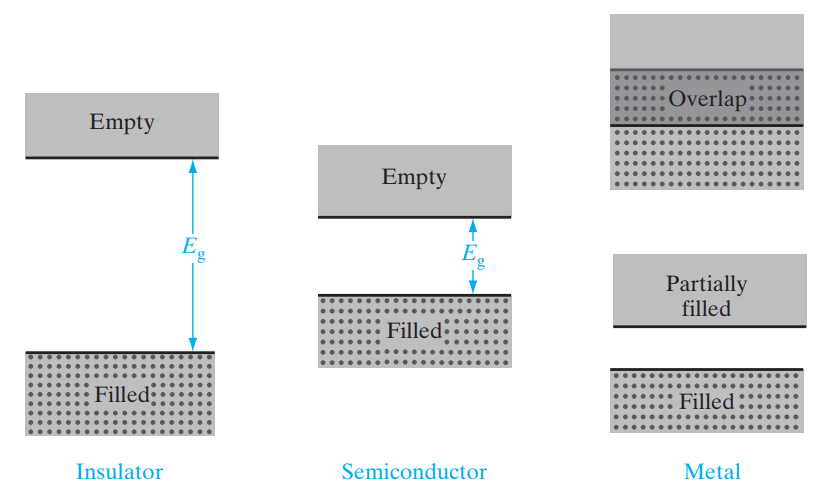
\includegraphics[width = 0.9\textwidth]{energy bands for materials}
%	\caption{}
	\label{fig:energy bands for materials}
\end{figure}



}
\Que{
Explain the difference in the recombination process between indirect and direct semiconductors. \hfill (\textit{final 2020}) \\or\\Explain why GaAs makes a better light emitting diodes while Si and Ge are better for transistors and IC applications. \hfill (\textit{midterm 2019})\\or\\Explain why indirect semiconductors are suitable for fabricationg transistors and ic applications \hfill (\textit{midterm 2021})
}
\Ans{
\begin{tabularx}{0.8\textwidth}{|X|X|}
\hline 
Direct semiconductors & Indirect semiconductors \\ 
\hline 
its band structure has a minimum at conduction band and a maximum at the valence band for \emph{the same k (momentum)} & its band structure has a minimum at conduction band and a maximum at the valence band for \emph{for different k (momentum)} \\ 
\hline
Electrons at conduction band can fall directly to empty states in valence band, giving off the energy difference as a \emph{photon} of light & Electrons at conduction band can't fall directly to  valence band,but they require a change in momentum, this can be done through some defect states within the band gap, it has first to lose energy through collisions with the crystals vibrating in the lattice, the quantization of the lattice vibration energy gives rise to the concept of \emph{phenon} particles. The participation of phenons and photons are necessary in the indirect transistors\\
\hline
Used in LEDs and lasers because \begin{enumerate}
\item the direct excitaion is favored energetically
\item the inverse reaction \textit{(direct recombination)}
 is highly probable\end{enumerate} & Used in transistor and IC application because current gain is high, since the carrires have to undergo a momentum change to recombine in transistor between emitter and collector, so they don't recombine easily which can reduce cureent gain.\\
\hline
\end{tabularx} 

\begin{figure}[H] 
	\centering
	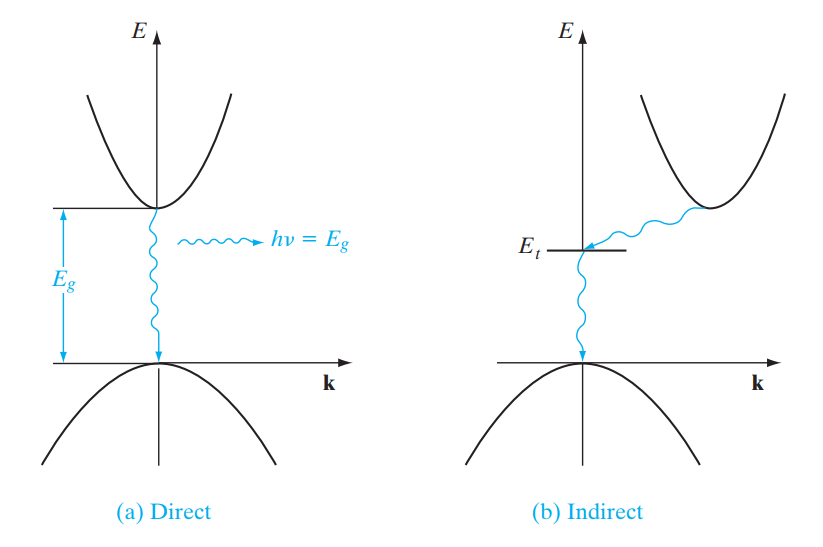
\includegraphics[width = 0.9\textwidth]{direct and indirect}
%	\caption{}
	\label{fig:direct and indirect}
\end{figure}

}

\Que{What is the disadvantage for using indirect semiconductors in LEDs and Laser applications?}
\Ans{
Most of the recombination energy goes into the vibrational energy of the crystal atoms which heats up the crystal.
}

\Que{
Explain electron hole pair in semiconductors
}
\Ans{
\begin{itemize}
\item As the temperature of a semiconductor increases from $0^{\circ}$ k some electrons in valence band receive enough thermal energy to be ejected to the conduction band, thus an electron hole pair is created.
\item After excitation to the conduction band, the electron is surrounded by a large number of unoccupied energy states, therefore they are free to move in many available empty states.
\item  in a filled band, all energy states are occupied, the net motion of electrons under the influence of external electric field is zero.
\item if an electron is removed, the net current will not be zero, this is equivalent to the motion of a positive charge in the opposite direction
\end{itemize}
}

\Que{
Explain briefly the meaning of effective mass
}
\Ans{
Due to the interaction of the electrons in the periodic potential of the lattice their wave-particle motion is not the same as that for electrons in free space.

We account for the influence of the by altering the value of the particle mass by $m^*$ 
$$\boxed{m^*=\frac{\hslash}{\frac{d^2E}{dk^2}}}$$
}

\Que{
Compare between \textbf{intrinsic} and \textbf{extrinsic} materials

}
\Ans{
\textbf{\textsc{Intrinsic materials}} :
\begin{itemize}
\item A perfect semiconductor lattice with no impurities or lattice defects.
\item There are no charge carriers at $0^{\circ}$
\item At higher temperature electron-hole pairs are generated
\item breaking of covalent bonds requires an energy equals to $E_g$
\item the position of free electrons and holes are not localized in the lattice, they are spread out over several lattice spacing and should be considered quantum mechanically by probability distribution for intrinsic materials.
\item $n=p=n_i$\\
$n$ : conduction band electron concentration\\
$p$ : valence band hole concentration\\
$n_i$ : intrinsic concentration

\item \emph{Generation rate} of electron-hole pairs must be equal to \emph{Recombination rate} $r_i = g_i $ , each of them is temperature dependent.
\item At any temperature rates of generation and recombination are proportional to the equilibrium concentration of $n_0$ and $p_0$ ($r_i = g_i = \alpha_r n_0 p_o = \alpha_r n_i^2$)
\end{itemize} 

\textsc{\textbf{Extrinsic materials}} :
\begin{itemize}
\item Semiconductor with impurities, it has additional carriers beside the intrinsic carriers
\item \emph{n type} :  an impurity from column \Romannum{5} (P,As,Sb) introduces an energy level near the conduction band.\\
At about $50^{\circ}$ k to $100^{\circ}$ k all the electrons in the impurities are donated to the conduction band ($n_0 >> n_i , p_0$)

\item \emph{p type} :  an impurity from column \Romannum{3} (Al, Ga, In) introduces an energy level near the valence band.\\
At about $50^{\circ}$ k to $100^{\circ}$ k all the electrons in the conduction band are accepted to the impurities from valence band ($p_0 >> n_i , n_0$)
\item in Ge (donor/acceptor) levels lies about 0.01 eV (below/above) (conduction/valence) bands
\item in Si corresponding values are 0.03 \& 0.06 eV
\end{itemize}


}

\Que{
Define Fermi Dirac distribution function
}
\Ans{
\begin{itemize}
\item Fermi Dirac distribution function is a function that gives the probability that an available energy state at E will be occupied by an electron at absolute temperature T $$ f(E) = \frac{1}{1+e^{(E - E_f)/KT}} $$
$E_f$ : Fermi level
$K$ : Boltzmann's constant = $8.62 \times  10^{-23} J/K$
\item Probability $f(E)$ means that above $E_f$ the states are filled. (electrons in the C.B)
\item Probability $1-f(E)$ means states below $E_f$ are empty . (holes in the V.B)
\item Due to the symmetrical nature of the distribution function about $E_f$ for all $T$. $$f(E_f + \Delta E) =1-f(E_f - \Delta E)$$
\end{itemize}

\begin{figure}[H] 
	\centering
	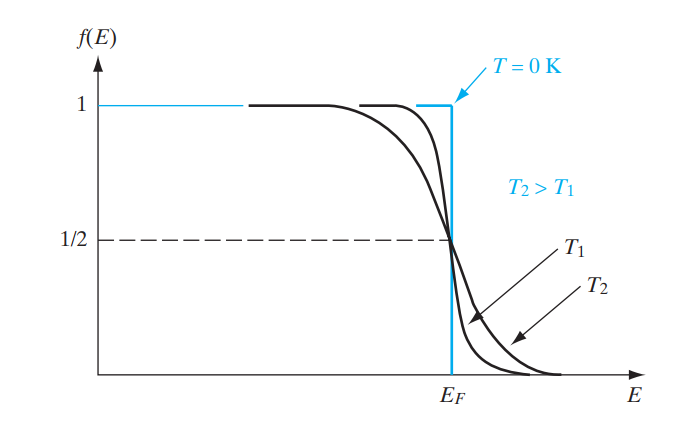
\includegraphics[width = 0.9\textwidth]{fermi}
%	\caption{}
	\label{fig:fermi}
\end{figure}

}

\Que{
Explain how Fermi level is an indication of the type of semiconductor and the amount of doping
}
\Ans{
\begin{enumerate}
\item \textbf{Intrinsic Materials}: Concentration of electrons in the conduction band \textbf{is equal to}concentration of holes in the valence band, therefor, the Fermi level is \textbf{in the middle} of the band gab.

\item \textbf{N type extrinsic Materials}:   Concentration of electrons in the conduction band \textbf{is higher than}concentration of holes in the valence band, therefor, the Fermi level is \textbf{near the conduction band}.

\item \textbf{P type extrinsic Materials}:   Concentration of electrons in the conduction band \textbf{is less than}concentration of holes in the valence band, therefor, the Fermi level is \textbf{near the valence band}.

\begin{figure}[H] 
	\centering
	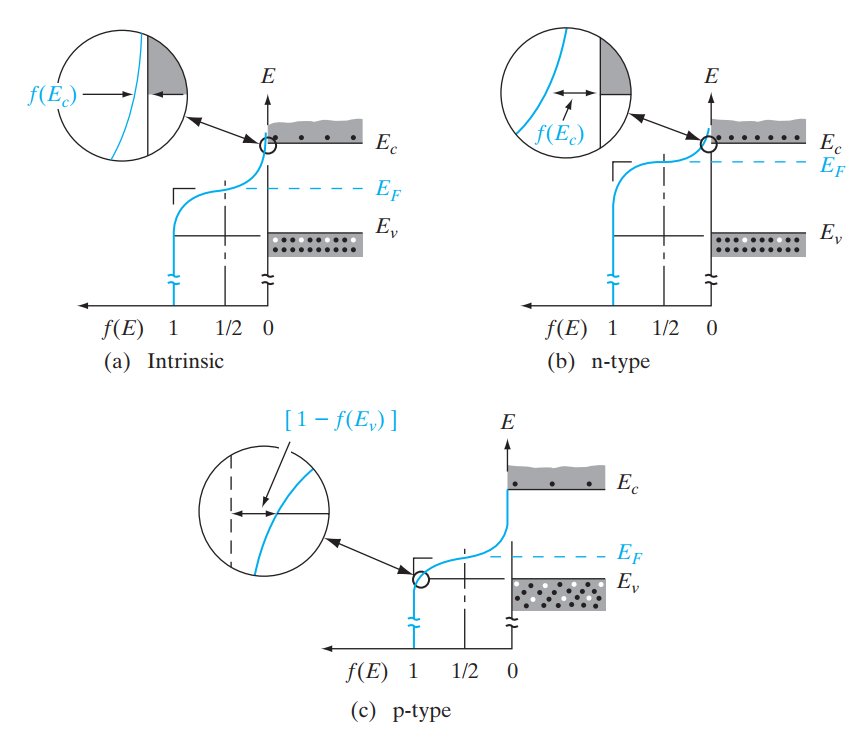
\includegraphics[width = 0.9\textwidth]{fermi for materials}
%	\caption{}
	\label{fig:fermi for materials}
\end{figure}

\end{enumerate}
}

\Que{
Prove that for any semiconductor material $n_0 p_0 = n_i^2$.
}
\Ans{
in the intrinsic semiconductor\footnote{Note that in intrinsic materials $E_f$ lies at intrinsic level $E_i$, near the middle of the band gap} 
\begin{align*}
&n_i = N_c e^{-(E_c - E_i)}\quad 
p_i = N_v e^{-(E_i - E_v)}\\
&n_i = p_i\\
&n_i p_i = N_c N_b e^{-(E_c - E_v)/KT} = N_c N_b e^{-(E_g)/KT}
\end{align*}


in the extrinsic semiconductor:
\begin{align*}
&n_0 = N_c e^{-(E_c - E_f)}\quad 
p_0 = N_v e^{-(E_f - E_v)}\\
&n_0 = p_0\\
&n_0 p_0 = N_c N_b e^{-(E_c - E_v)/KT} = N_c N_b e^{-(E_g)/KT}
\end{align*}
so $\displaystyle n_0 p_0 = n_i^2 $ for any semiconductor.
}

\Que{
In an n type material, draw the relation between majority carrier concentration and the temperature. Indicate the optimum temperature range for device operation and give reasons for this choice \hfill \textit{(midterm 19)(midterm 20)}
}
\Ans{
\emph{At low temperature(high $\frac{1}{T}$)}
\begin{itemize}
\item Very small intrinsic electron-hole pairs
\item Donor electrons bound are bounded to donor atoms.
\end{itemize}
\emph{At temperature increases ($\frac{1}{T}$ decreases)}
\begin{itemize}
\item Donor electrons are donated to the conduction band until all donors are ionized
\item Electron concentration remains constants at $n_0 = N_d$, this is why this region is the optimum region for device operation.
\end{itemize}
\emph{At large temperature (small $\frac{1}{T}$)}
\begin{itemize}
\item more electrons are donated due to intrinsic electron-hole pair generation. $n_o = n_i >> N_d$
\end{itemize}

\begin{figure}[H] 
	\centering
	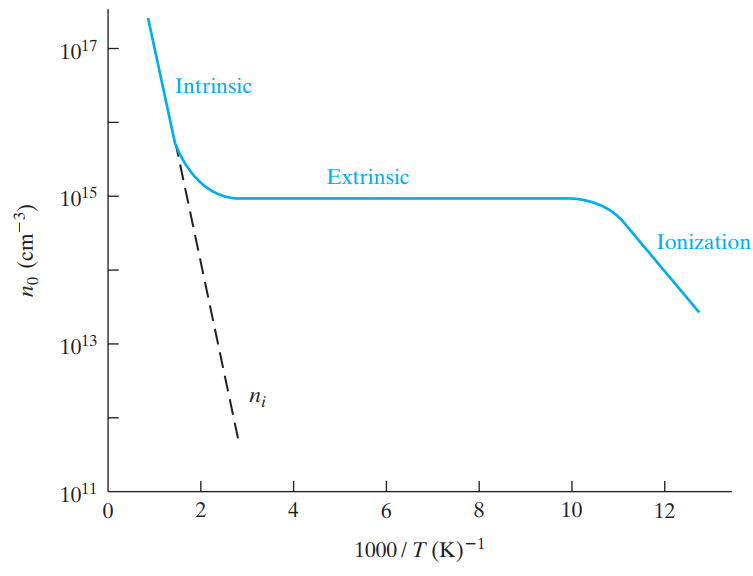
\includegraphics[width = 0.9\textwidth]{concentration and temp}
%	\caption{}
	\label{fig:concentration and temp}
\end{figure}


}

\Que{
A si sample is doped with Ga atoms (trivalent material) at a concentration of $10^6$ $\text{atoms/cm}^{3}$. Calculate both majority and minority carriers concentration at $300^{\circ}$ k and energy difference between Fermi level and intrinsic level. \hfill \textit{(midterm 19)(final 20)}
}

\Ans{
Given $(T=300^{\circ} k, n_i = 1.5 \times 10^{10} \text{cm}^{-3}, KT=0.0259 eV)$
\begin{align*}
p_0 &\approx N_a = 10^{16} \text{atoms/cm}^{-1}\\
p_0 &= n_i e^{(E_i - E_f)/KT}\\
\frac{p_0}{n_i}&= e^{(E_i - E_f)/KT}\\
\ln \left( \frac{p_0}{n_i} \right) &= \frac{E_i - E_f}{KT}\\
E_f - E_i &= - KT \ln\left(\frac{p_0}{n_i}\right)\\
&= - 0.0259\ln \left( \frac{10^{16}}{1.5 \times 10^{10}} \right)\\
&= -0.0347 eV
\end{align*}
}

\Que{
Illustrate compensation and space charge neutrality process.
}
\Ans{
\begin{itemize}
\item if a semiconductor has donors and acceptors and $N_d>N_a$\\
the material is n type and Fermi level is near the conduction band 

\item The filling of the $E_a$ states occurs at the expense of the donated conduction band electrons

\item If the acceptors states are filled with valence band electrons the holes are then filled due to recombination with conduction band electrons, therefore the resultant concentration of conduction band electrons will be $N_d - N_a$

\item this process is called compensation

\item if the materials remains electrostatically neutral $$P_0 + N_d^+ = n_0 + N_a^-$$ 
For n type material $n_0 >> p_0 \quad\quad \therefore n_0 = N_d - N_a$\\
For p type material $p_0 >> p_0 \quad\quad \therefore p_0 = N_a - N_d$\\
\end{itemize}
}

\Que{
A Ge sample is doped with $5 \times 10^{13}$ Sb atoms/$\text{cm}^3$ using the requirements of charge neutrality calculate the electrons concentration $n_0$ at $300^{\circ}$ k.\\Given ($n_i \text{for Ge} = 2.5 \times 10^{13} \text{atoms/cm}^3$)
}
\Ans{
\begin{align*}
n_0 &= p_0 + N_d  \tag{$\times n_0$}\\
n_0^2 &= n_i^2 + N_d n_0 \\
n_0^2 - N_d n_0-n_i^2 &= 0  \tag{Solve using quadratic formula}\\
x&=\frac{-b \pm \sqrt{b^2 -4ac}}{2a} \tag{$a=1, b=-N_d, c=-n_i^2$}\\
n_0 &= \frac{N_d \pm \sqrt{N_d^2 +4n_i^2}}{2}\\
n_0 &= \frac{5*10^{13} \pm \sqrt{(5*10^13)^2 +4(2.5*10^{13})^2}}{2}\\
&= 3.036*10^{13} \text{atoms/cm}^3 \tag{The negative solution is refused}\\
\end{align*}
}

\Que{
How long does it take an average electrons to drift $1\mu m $in pure Si ate electric field = 100 v/cm ($\mu_m = 1350 \text{cm}^2/V.s$)
}
\Ans{
\begin{align*}
v = \mu_m E = 1350*100=135*10^{3} \text{cm/s}
t = \frac{d}{v} = \frac{1 * 10^{4}\text{cm}}{135*10^{3}\text{cm/s}} = 7.41 \times 10^{-10} \text{s}.
\end{align*}
}



\Que{
How does the higher values of electric field affect the carriers velocities in different types of semiconductor materials. \hfill \textit{(final 2021)(midterm 2022)}

}


\Ans{\begin{itemize}
\item At low value of E $$J=\sigma E$$ 

\item For  $E>10^{3} V/m$, $\sigma$ becomes dependent on E.\\This is called hot carrier effect, in this case the carrier drift velocity $V_d$ is comparable to the thermal velocity $V_{th}$ 
$$\frac{1}{2}mv_{th}^2 = KT$$
$$v_{th} =\sqrt{\frac{2KT}{m}} = 10^{7} \text{cm/s} $$
An upper limit of drift velocity $V_d$ is reached near $V_d = V{_th}$



\item At this point any added energy is transferred to the lattice rather than increasing the carrier velocity, this limit is called the scattering it velocity.

\item In GaAs, Electron velocity decreases at high fields giving negative conductivity. 

\begin{figure}[H] 
	\centering
	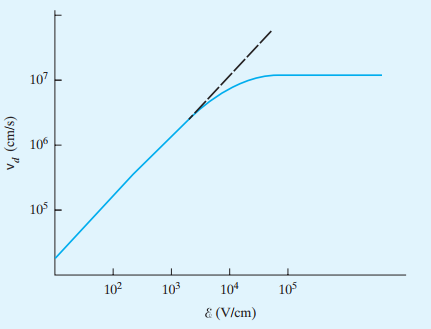
\includegraphics[width = 0.6\textwidth]{vd saturation}
%	\caption{}
	\label{fig:vd saturation}
\end{figure}
\end{itemize}
}\Que{
Explain how does the carriers mobility in semiconductors varies with temperature, doping concentration and high field. \hfill (final 2020)(midterm 2022)
}
\Ans{
\begin{itemize}
\item At low temperature, \emph{Impurity scattering} is dominant, as slow electrons are likely to be scattered more strongly by the interaction with the charged ions

\item By increasing the temperature, \emph{impurity scattering} becomes less effective,therefore the mobility increases up to certain temperature.

\item At certain temperature, \emph{lattice scattering} becomes dominant, this type of scattering is caused by the thermal vibrations,therefore the mobility decreases $$\frac{1}{\mu} = \frac{1}{\mu_1} + \frac{1}{\mu_2} + \cdots $$

\item Increasing doping increases \emph{impurity scattering}, therefore the mobility decreased.

\begin{figure}[H] 
	\centering
%	\subfloat{{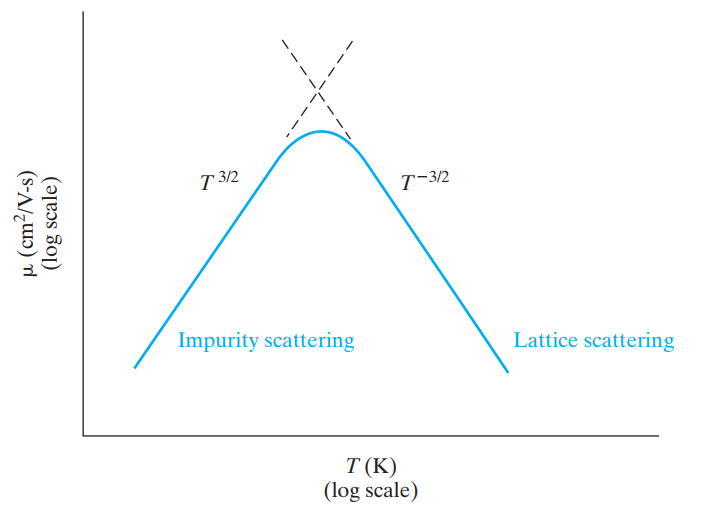
\includegraphics[width = 0.4\textwidth]{scattering} }}%
%    \qquad
%    \subfloat{{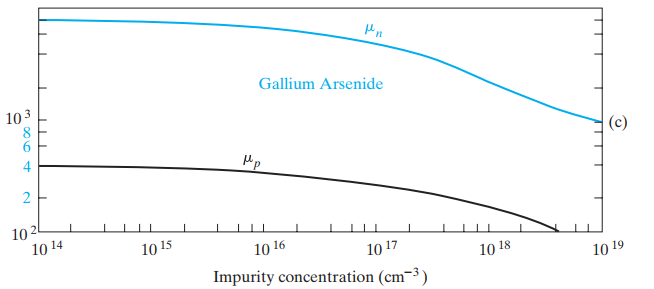
\includegraphics[width = 0.4\textwidth]{mobility temp} }}
	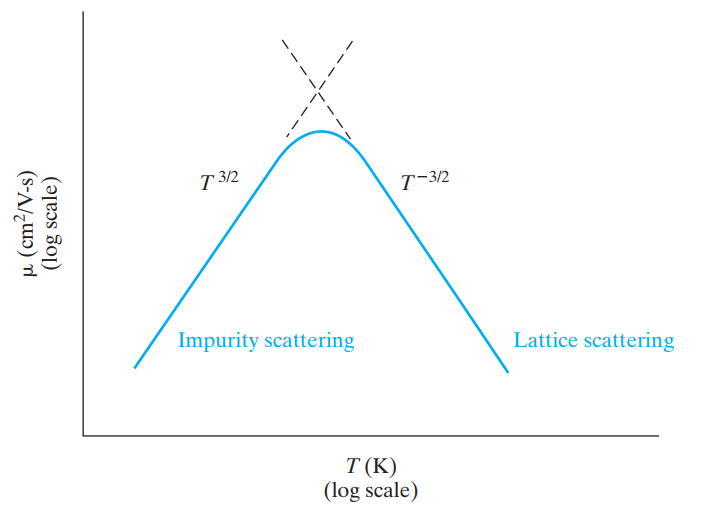
\includegraphics[width = 0.65\textwidth]{scattering}
	\caption{Approximate temperature dependence of mobility with both lattice and impurity scattering.}
	\label{fig:scattering}
\end{figure}


\begin{figure}[H] 
	\centering
%	\subfloat{{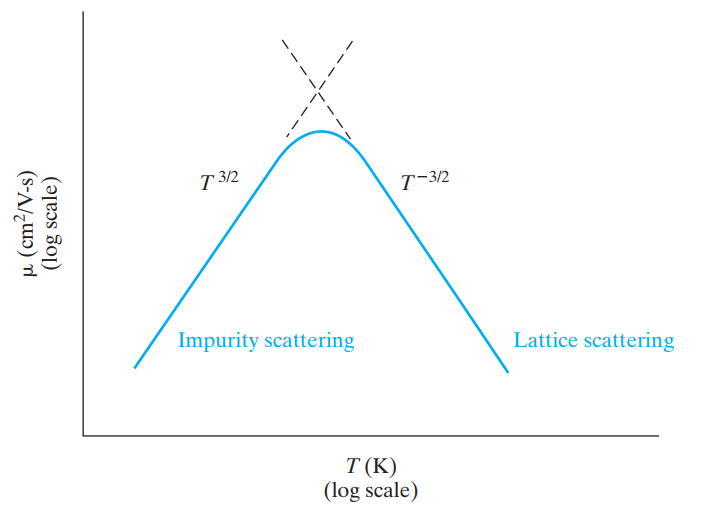
\includegraphics[width = 0.4\textwidth]{scattering} }}%
%    \qquad
%    \subfloat{{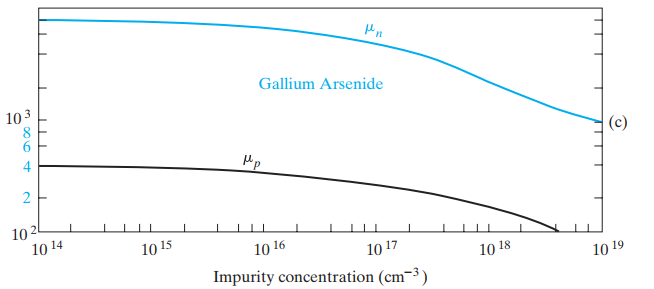
\includegraphics[width = 0.4\textwidth]{mobility temp} }}
	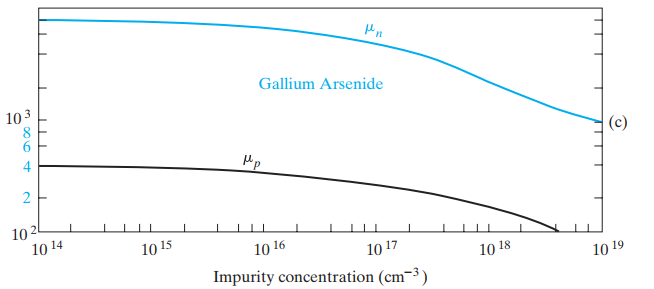
\includegraphics[width = 0.65\textwidth]{mobility temp}
	\caption{Variation of mobility with total doping impurity concentration}
	\label{fig:mobility temp}
\end{figure}


\end{itemize}
}

\Que{
Based on the \emph{Hall effect} derive expressions for the majority carriers concentration, resistivity and carrier mobility \hfill \textit{(midterm 2020)(midterm 2021)} 
}
\Ans{
If a magnetic field is applied perpendicular to the direction in which holes drift in a p type bar, a force in the -ve y direction results and equals to $$F_y = qE_y - v_x \, B_Z$$
since the net force equals zero 
\begin{align*}
qE_y &=q\, v_x \, B_Z\\
E_y &=\, v_x \, B_Z \tag{$v_x = \dfrac{J_x}{qp_0}$}\\
E_y &=\, \frac{J_x}{qp_0} \, B_Z \tag{let $R_H = \dfrac{1}{qp_0}$}\\
E_y &=\, R_H \, J_x \, B_Z\tag{$R_H$ is the hall coeffecient}\\
\end{align*}
\begin{align*}
&P_0 = \frac{1}{q\,R_H}=\frac{J_x\,B_z}{q\,E_y} = \frac{\frac{I_x}{w\,t}\,B_z}{q\frac{V_{AB}}{w}} = \frac{I_x\,B_z}{q\,t\,V_{AB}} \tag{1}\\
&\rho = \frac{RA}{L} = \frac{Rwt}{L}= \frac{V_{CD}/I_x}{L/wt}\\
&\mu_p = \frac{\rho}{qp_0} = \frac{1/\rho}{\rho/(1/\rho R_H)} = \frac{R_H}{\rho}\\
\end{align*}
from (1) the sign of $V_{AB}$ indicates the type of the semiconductor, if $V_{AB}>0\quad \Rightarrow$ p-type -   if $V_{AB}<0\quad \Rightarrow$ n-type.


}
\Que{
In n-type semiconductor derive expressions for the \emph{drift current intensity} and the \emph{electrons mobility} .
}
\Ans{
\begin{itemize}
\item At room temperature, the thermal motion of an electron may be visualized as random scattering from lattice vibration, impurities, other electrons and defects.

\item There are no net motion of the group of n electrons/cm\textsuperscript{3} over any period of time .

\item if an electric field $E_x$ is applied, the force of the field on the n electrons/cm\textsuperscript{3} is $$-nqE_x = \left. \frac{dp_x}{dt}\right|_{\text{field}} \quad \quad p_x = (mV_x)\times n$$
\item $p_x$ is the total momentum of the group
\item At steady state, the net acceleration is balanced by the deceleration of collision process.
\item if the collisions are random, there will be a constant probability of collisions at any time for each electron.
\item Rate of decrease of $N(t)$ at any time is proportional to the number left unscattered.

%
\begin{align*}
 -\frac{dN(t)}{dt} \propto N(t) \quad ,\quad
 -\frac{dN(t)}{dt} = \frac{1}{\Bar{t}} N(t) \quad ,\quad
 N(t) = N_0 e^{-t/\Bar{t}}\\
\end{align*}




$N(t)$ : the number of electrons which have not undergo a collision by time $t$.
$N_0$ : group of electrons at $t=0$. 
$\Bar{t}$ : mean time between scattering events.

\item Probability that any electron has a collision in the time interval 
$dt = \dfrac{dt}{\Bar{t}}$
\item Differential change in $p_x$ due to collisions is $$dp_x=-p_x\frac{dt}{\Bar{t}}$$

\item the rate of change of $p_x$ due to the deceleration effect of collisions is $$\frac{dp_x}{dt}=-\frac{p_x}{\Bar{t}}$$.

\item The net acceleration is zero 
\begin{align*}
\left. \frac{dp_x}{dt}\right|_{acc} + \left. \frac{dp_x}{dt}\right|_{decc} = 0\\
-nqE_X - \frac{p_x}{\Bar{t}} = 0\\
p_x = -nq\Bar{t}E_x
\end{align*} 

\item The average momentum $\displaystyle <p_x> = \frac{p_x}{n} = -q\Bar{t}E_x$.

\item The average velocity $\displaystyle <v_x> = \frac{<p_x>}{m^*_n} = -\frac{q\Bar{t}{m^*_n}}E_x$

\item The current density $$ J_x = -qn<v_x> = \frac{nq^2\Bar{t}}{m^*_n}E_x$$ but $ J_x - \rho E_x$ 
$$\therefore \rho = \frac{nq^2\Bar{t}}{m^*_n}$$
but $\rho = qn\mu_n$
$$\therefore \mu_n = \frac{q\Bar{t}{m^*_n}}= -\frac{<v_x>}{E_x} \quad \text{(cm\textsuperscript{2}/V.sec)}$$
$$\therefore J_x = q_n \mu_n E-x \text{ for electrons}$$

$$\therefore j_x = q(n\mu_n+p\mu_p)E_x = \rho E_x \text{ for both electrons and holes}$$


\end{itemize}
}

\end{large}
\end{document}
















